\documentclass[12pt]{article}
%% Package Declarations:
\usepackage[a4 paper, margin=1in]{geometry}
\usepackage[english]{babel}
\usepackage[utf8]{inputenc}
\usepackage{subcaption}
\usepackage{pdfpages}
\usepackage{longtable}

\usepackage{times}
\usepackage[T1]{fontenc}

\usepackage[compact]{titlesec}
\usepackage{graphicx}
\usepackage{enumitem}
\usepackage{colortbl}
\usepackage{float}
\usepackage{multirow}

\usepackage{acronym}
\usepackage{tocloft}
\usepackage{setspace}
\usepackage{url}
\usepackage[hidelinks,linktoc=all]{hyperref}
\usepackage[backend=biber,style=ieee]{biblatex}

%% Configs

\urlstyle{same}

\onehalfspacing

\definecolor{sea}{RGB}{175,255,215}

\DeclareUnicodeCharacter{0301}{\'\i}

\addto\captionsenglish{
 \renewcommand{\contentsname}
 {Table of Contents}
}

\addbibresource{./references.bib}

% \setlength{\parindent}{0em}
% \setlength{\parskip}{1.5pt}


\begin{document}

\begingroup
  \fontsize{12pt}{14pt}\selectfont
  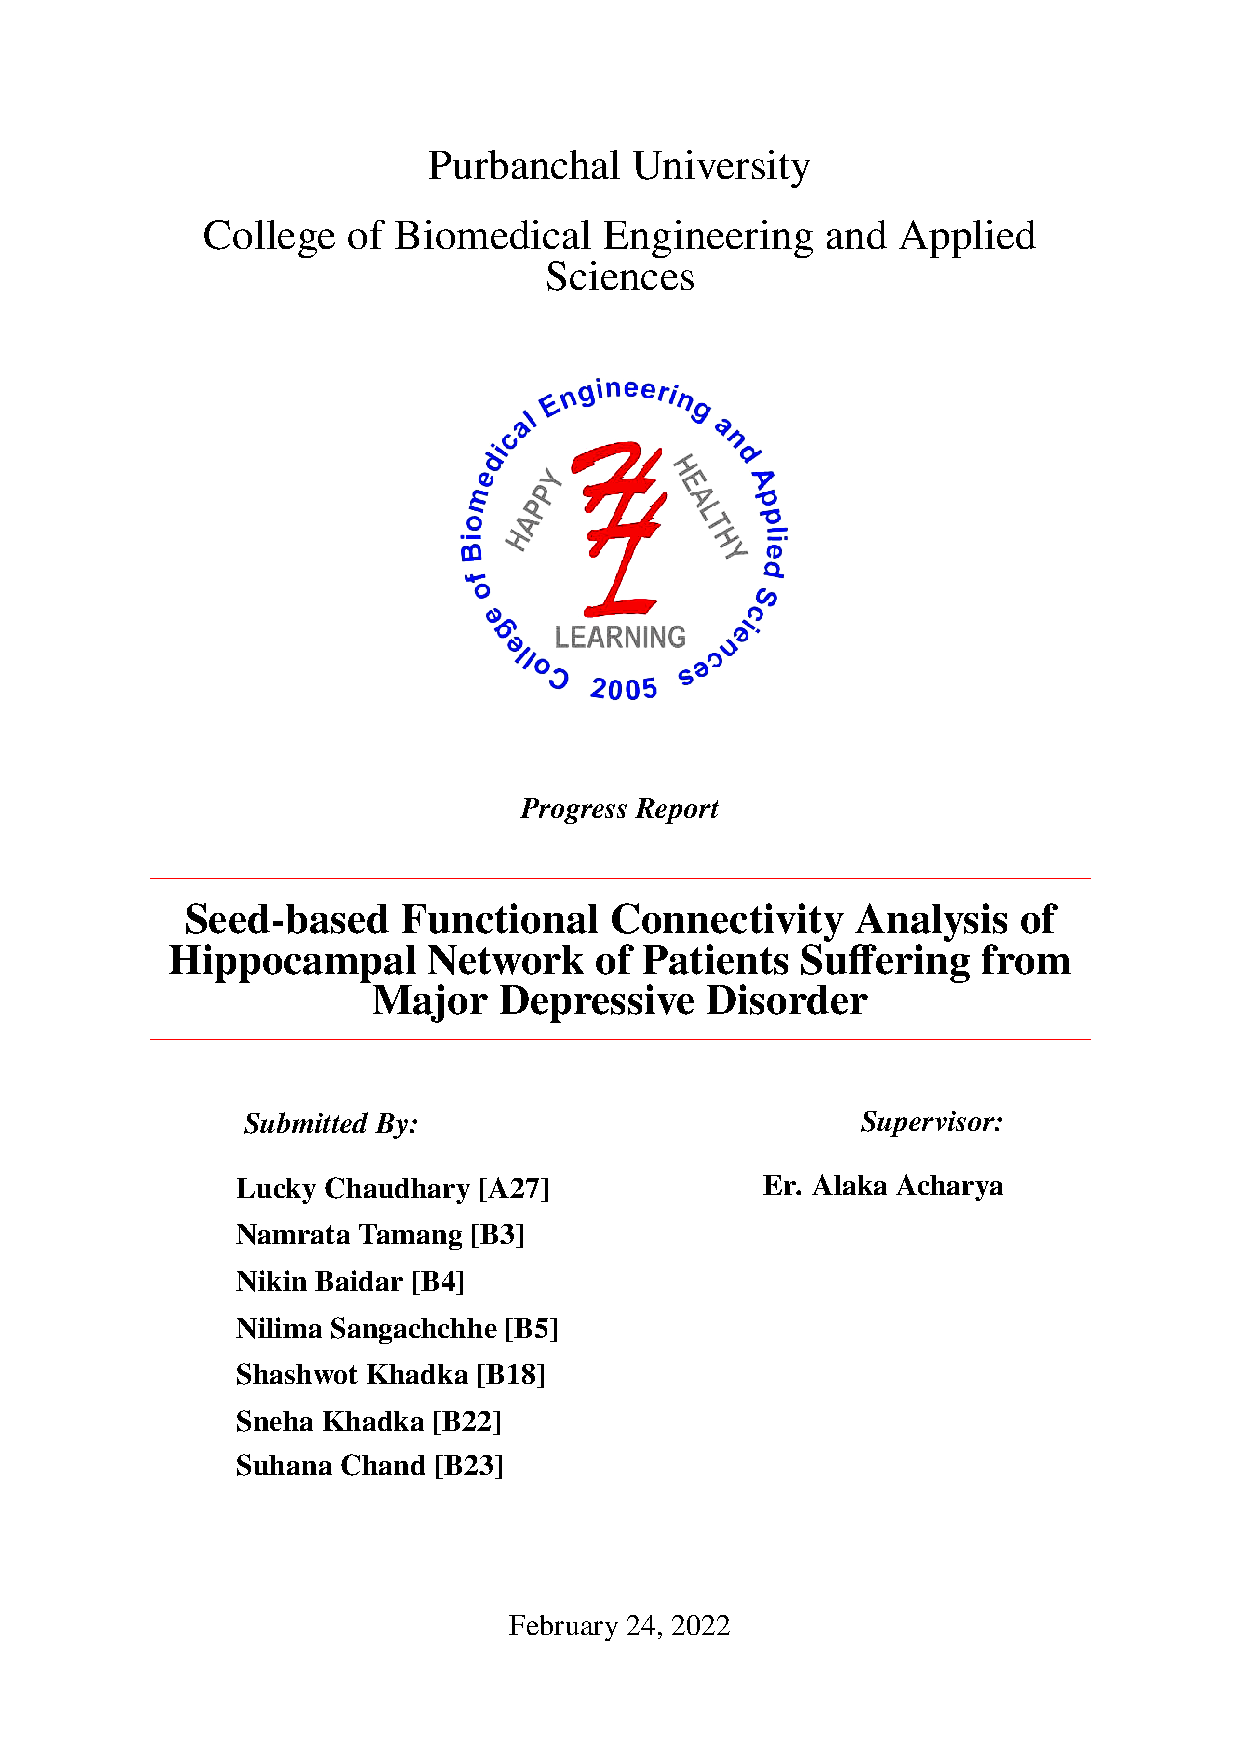
\includepdf[pages=-]{./titlepage.pdf}

% preface
\pagenumbering{roman}
\clearpage
\setcounter{page}{1}
\hskip180pt {\textbf{\centering \Large Preface} }
\vskip40pt
\addcontentsline{toc}{section}{Preface}

\noindent
The basis for this project stemmed from the fact that not many
researches have been conducted in Nepal regarding the diagnosis of
mental disorders. Nonetheless, in other countries, many researches and
studies have been conducted regarding the functional connectivity of
different brain regions in depression and other mental
disorders. However, till date, there is no solid evidence that could
be used for the clinical diagnosis of mental disorders. Our project
intends to review past researches and keep up with the studies related
to Major Depressive Disorder and brain functional connectivity. In
addition to that, we have selected hippocampal circuity as the region
of interest for our purposes and the overall project is going to
revolve around how functional connectivity of hippocampal network in
MDD patients differ from that of healthy people.

\hspace*{133mm}\textbf{\textit {$-$ Authors}}
\newpage

%abstract
\hskip180pt {\textbf{\centering \Large Abstract} }
\vskip2pt
  \addcontentsline{toc}{section}{Abstract}

\newpage

\thispagestyle{empty}
\addcontentsline{toc}{section}{List of Figures}
\listoffigures

\thispagestyle{empty}
\addcontentsline{toc}{section}{List of Tables}
\listoftables
\newpage

% Abbreviations

\begin{center}
  \section*{Abbreviations}
  \addcontentsline{toc}{section}{Abbreviations}
\end{center}

\begin{acronym}
  \acro{AFNI}{Analysis of Functional Neuroimages}
  \acro{BDI}{Beck Depression Index}
  \acro{BOLD}{Blood Oxygen Level Dependent}
  \acro{CSF}{Cerebrospinal Fluid}
  \acro{fMRI}{Functional Magnetic Resonance Imaging}
  \acro{GM}{Gray Matter}
  \acro{HCs}{Healthy Controls}
  \acro{MDD}{Major Depressive Disorder}
  \acro{MR}{Magnetic Resonance}
  \acro{rs}{Resting State}
  \acro{rsFC}{Resting-state Functional Connectivity}
  \acro{SCA}{Seed-based Correlation Analysis}
  \acro{sMRI}{Structural Magnetic Resonance Imaging}
  \acro{SPM}{Statistical Parametric Mapping}
  \acro{WM}{White Matter}
\end{acronym}

\newpage

\begingroup
  \fontsize{12pt}{12pt}\selectfont

% table of contents
\vskip -10pt
\enlargethispage{\baselineskip}
\thispagestyle{empty}
\addcontentsline{}{}{}
\tableofcontents

\endgroup
\newpage

\pagenumbering{arabic}
\clearpage
\setcounter{page}{1}

\section{Introduction}

So, based on our objective proposed, this refers to the progress
report of our project till date along with the future works to be
performed that completely meet our aims.

Functional MRI is well established as a method for the detection and
delineation of regions of the brain that change their level of
activation in response to specific stimulus. fMR imaging modality
is sensitive to fluctuations in the BOLD signal which reflects
neuronal activation, or neuronal activity.


\subsection{Background}

The specific objective of this project is to perform seed-based
functional connectivity analysis to study how the normal function of a
particular area of a healthy brain gets disrupted in diseased
conditions. Major Depressive Disorder being one of the major mental
health illnesses in our country, this project aims to analyze the
functional changes in the brain of MDD patients compared to healthy
controls. Furthermore, in our literature review, it was found that the
hippocampus of the brain is one of the major regions affected by a
variety of neurodegenerative and mental disorders. For this reason, we
aim to assess the functional connectivity of the hippocampal region of
the brain.

\subsection{Rationale}

The absence of biological markers makes it exceptionally difficult for
neurologists to diagnose a person with a psychiatric disorder. The
diagnostic procedures that are the gold standard for the diagnosis of
neurodegenerative and psychiatric disorders, in the present day, are
wholly based on behavioral observations and patient reported symptoms,
both of which do not have a molecular or radiological basis. Although
there have been countless studies conceptualizing the possibility of
implementation of various functional imaging modalities for
deciphering the etiology and the functional effects of various mental
disorders, the findings from these studies do not appear amongst the
diagnostic criteria. A critical barrier to the clinical translation of
many such findings is the reverse inference fallacy.

The information from structural radiology modalities describe the
shape, size and integrity of brain structure, but they do not provide
any information about the brain function. Nonetheless, as we will
discuss in the coming sections of this progress report, combining
structural MRI and functional MRI can be a promising technique to
characterize normal and abnormal brain function, which can act as an
auspicious biomarker for neurodegenerative or psychiatric disorders to
determine the risk, progression and therapeutic effectiveness. This
project can lay the foundations for further research and development
in this particular field.


\newpage
\section{Methodology and Review on Individual Tasks}

\subsection{System Setup}%
\label{sub:system_setup}
\addtocontents{toc}{\protect\setcounter{tocdepth}{2}}

For the following project, the primary software tool that we will use
for functional connectivity analysis is AFNI. AFNI (Analysis of
Functional NeuroImages) is an open-source software, distributed
freely under the GNU General Public License.  AFNI is used for
processing, analyzing and displaying several MRI modalities such as
anatomical MRI, functional MRI (FMRI) and diffusion weighted (DW)
data. AFNI runs virtually on any UNIX based system such as macOS and
GNU~Linux. For financial reasons, we opted to install GNU~Linux. Along
with AFNI, we will also use SPM (Statistical Parametric Mapping) which
is an image processing package in GNU Octave. GNU Octave, and all of
its associated programs, is freely distributed under the terms of the
GNU General Public License.

GNU Linux is an open-source Unix-like operating system. The Linux
kernel is licensed under the terms of GNU General Public License
version 2 (GPL-2.0). Popular Linux distributions include Ubuntu,
Linux Mint, Fedora, and Arch. After we collected the SSDs that we
requested for, we installed various linux distributions, namely
Ubuntu, Linux Mint and Arch Linux. After installation of Linux, we
installed AFNI and other related software on our Linux systems.

\subsubsection{Runtime Environment}%
\label{ssub:runtime_environment}

Here is a list of the major softwares used, along with their version
information, during the runtime for the codes and results included in
the following report:

\begin{itemize}[noitemsep]
  \item Operating System: Arch Linux x86\_64, kernel version
    5.16.8-arch1-1
  \item AFNI, version AFNI\_22.0.03 `Hadrian'
  \item GNU Octave, version 6.4.0


\end{itemize}

\subsection{Data Acquisition}%
\label{sub:data_acquisition}

The functional and anatomical MR images for the progression of this
study were acquired from the SRPBS Multidisorder MRI Dataset. The
datasets included were obtained from the DecNef Project Brain Data
Repository, which is a repository of neurological images gathered by a
consortium as a part of the Japanese Strategic Research Program for
the Promotion of Brain Science supported by the Japanese Advanced
Research and Development Programs for Medical Innovation (AMED).
Furthermore, the MR datasets included in this repository were
diagnosed by trained and experienced neurologists, which assures that
our study will be tilted more towards accuracy and efficiency
\cite{dataset}. We acquired functional MR as well as T1 weighted
images of subjects from two distinct categories. The first set of
subjects are categorized as healthy controls, and the second set of
subjects are categorized as those who are suffering from major
depression. The subjects from the first category, i.e.~healthy
controls will be referred to as ``HC'' and the subjects from the
second category, i.e.~depressed subjects will be referred to as ``MDD
patients''.

\newpage
\subsection{Data Selection}%
\label{sub:data_selection}

The SRBPS dataset originally had the MR images of more than 1400
volunteers. All of these volunteers had undergone a standardized
clinical evaluation protocol, which involved a general and
neurological evaluation. This opts for the accuracy of our study.

The following is a brief summary of the tasks performed during this
step:

\begin{table}[H]
  \centering
  \begin{tabular} {| m{3.3cm} | m{11.5cm} | }
    \hline
    \multicolumn{2}{|c|}{Selection of Data} \\ \hline
    Status during the reporting period   & Completed   \\ \hline
    Actions &
    Out of the data of 1400 volunteers from the SRBPS dataset, 15
    healthy controls (diagnosis~0) and 15 depressed patients
    (diagnosis~2) were manually selected by just eyeballing the data
    sheet included in the data acquired from the SRBPS public
    repository.  \\ \hline

    Decisions &
    \begin{itemize}

      \item The datasheet contained data of volunteers from various
        different site. Subjects of either sex, male or female, were
        selected from only one specific site, HUH in particular. The
        reason behind this was to make sure that the images that we
        will be working on were acquired from the same MRI scanner.
        This ensure consistency of data.

      \item Majorly depressed patients were labeled with a BDI (Beck
        Depression Index) greater than 30.~So subjects having
        BDI $>$ 30 were only selected.

      \item Trying to acquire data of people from a certain age group
        was a failure because there was not just enough data of the
        volunteers with BDI $>$ 30. So we had to settle with subjects
        of the age group 20 to 50.

    \end{itemize} \\ \hline

    Testing \& Verification &
    Once we had the subjects decided, two statistical tests were
    performed:
    \begin{enumerate}[noitemsep]
      \item Chi-square test
      \item t-test
    \end{enumerate}

    Chi-square test was performed to check the goodness of fit between
    healthy controls and depressed subjects based on sex and the
    t-test was performed to check the goodness of fit based on age. \\ \hline
  \end{tabular}
\end{table}

The results of both t-test and the chi-square tests were positive
(Appendix A), therefore we concluded that the subjects we selected for
both categories, HC and MDD were well matched.

\newpage
\subsection{Data Preparation}%

After we finalized the subjects on which we will be working on, the
image data that we acquired were converted into appropriate formats
that could be used for further processing. The original image data
that we acquired were in DICOM image format.

\begin{table}[H]
  \centering
  \begin{tabular} {| m{3.3cm} | m{11.5cm} | }
    \hline
    \multicolumn{2}{|c|}{Conversion of image data from DICOM format to
    NIfTI format} \\ \hline
    Status during the reporting period   & Completed   \\ \hline
    Actions &
    Created a BASH script to add the NIfTI extension i.e.~``.nii'' in
    order to convert the image data of 15 HC as well as 15 MDD
    patients from DICOM format to NIfTI format. (Appendix B) \\ \hline

    Decisions &
    \begin{itemize}

      \item A DICOM file is an image saved in Digital Imaging and
        Communication in Medicine (DICOM) format.  DICOM format is an
        internationally accepted format in which medical images are
        scanned, stored, retrieved and shared.

      \item However, different scanner manufacturers extend the DICOM
        format in a variety of ways, which often results in
        duplication of information and incompatibilities between
        softwares. The Neuroimaging Informatics Technology Initiative
        (NIfTI) file format has become the standard for neuroimaging
        studies. In addition to that, the software tools (AFNI and
        SPM) that we will be using for image processing, analysis and
        visualization require images to be stored in the NIfTI file
        format. For these reasons, the original datasets which were in
        the DICOM format were converted into NIfTI format.

    \end{itemize} \\ \hline

    Testing \& Verification &
    The images after conversion to NIfTI were opened in AFNI to verify
    that it could understand and render the image data in its
    interface. \\

    \hline

  \end{tabular}
\end{table}

Furthermore, once the image data were converted into the NIfTI format,
which could be understood by a variety of software tools that we use,
the multiple 3D rsfMRI image data was converted into a single 4D BOLD
data for each subject from either category.

\begin{table}[H]
  \centering
  \begin{tabular} {| m{3.3cm} | m{11.5cm} | }
    \hline
    \multicolumn{2}{|c|}{Conversion of 3D fMRI image into 4D BOLD Data} \\ \hline
    Status during the reporting period & Completed   \\ \hline
    Actions &
    A file conversion tool called dcm2nii with a graphical user
    interface was used to select all the 3D rsfMRI volumes to create a
    compressed file format containing the 4D BOLD data.  \\ \hline

    Decisions &
    \begin{itemize}

      \item Unlike an anatomical MR image which is a single volume, a
        functional MR image is acquired in blocks, where each block
        represents the functional MR signal acquired at a given time.
        It is essential to merge these multiple 3D functional MR image
        volumes into a single 4D functional MR image, where time is
        the fourth dimension.

    \end{itemize} \\ \hline

    Testing \& Verification &
    This step didn't require any testing. Nonetheless, the compressed
    file was decompressed and its size was checked to verify it was
    greater than 0 bytes.  \\
    \hline
  \end{tabular}
\end{table}

After these two steps, our image data for both HCs as well as MDD
patients were prepared for further processing.

\newpage
\subsection{Skull Stripping}

Since high resolution structural images contain considerable amounts
of non-brain tissue such as eyeballs, bone, skin, amongst other
tissues. Skull stripping improves the quality and accuracy of the
normalization and templates that will be created for skull-stripped
images. The skull stripping was achieved in AFNI. The skull stripping
process completes in the following steps:

\begin{table}[H]
  \centering
  \begin{tabular} {| m{3.3cm} | m{11.5cm} | }
    \hline
    \multicolumn{2}{|c|}{Extraction of the brain tissue} \\ \hline
    Status during the reporting period   & Completed   \\ \hline
    Actions &
    AFNI provides a skull stripping tool called 3dSkullStrip. A shell
    script was created to implement this 3dSkullStrip program to
    extract the brain tissues in T1 weighted images of each subject
    from either category. (Appendix C) \\ \hline

    Decisions &
    \begin{itemize}

      \item After data preparation, our next step would be
        segmentation of various brain structures from the brain. But
        before doing just that, the brain tissues must be extracted by
        removing the surrounding skull in order to isolate the brain
        tissue from non-brain tissue from an MRI image of a brain.

      \item We decided that it would be better to strip the skull
        from T1 images in order to exclude gross spatial image
        non-uniformity artifacts and to reposition the brain in a
        reasonable manner.

    \end{itemize} \\ \hline

    Testing \& Verification &
    The generated files were visualized in the AFNI interface. The
    following figures represent a basic visualization of the results
    for an axial image with z at 0.404~mm.


    \begin{minipage}{.6\textwidth}
    \begin{figure}[H]
      \captionsetup{singlelinecheck = false, justification=justified}
      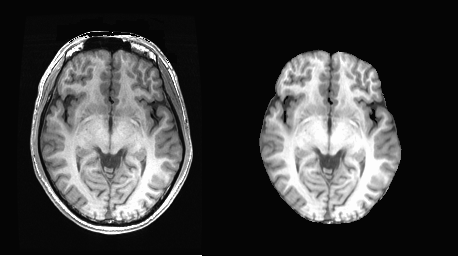
\includegraphics[width=\linewidth]{./.img/test.png}
      \caption{Axial Brain Image with Skull and without skull}%
      \label{fig:axial_brain_image_with_skull}
    \end{figure}
    \end{minipage}

    \\ \hline

  \end{tabular}
\end{table}

Once the brain tissue is extracted from the T1 image, we proceed to
image segmentation.

\newpage
\subsection{Image Segmentation}

Image segmentation is the process of partitioning a digital image into
multiple image segments, or image regions which essentially are a
similar set of pixels. The primary goal of image segmentation is
feature extraction, to simplify and change the representation of an
image into something that is more meaningful and easier to analyze.
Most, if not all, of the analysis of medical images requires some form
of segmentation or feature extraction. Segmentation makes it easier
to analyze any given image, as it distinguishes structures, regions or
tissue classes of interest from other details in the image.
Segmentation depends on a variety of features that are contained in
the image. The features can be either color or texture or something
else. The primary reason for image segmentation for our purposes is to
reduce the information for easy analysis.

For our purposes, the image segmentation part involves segmentation of
the gray-matter, white-matter and the cerebrospinal fluid in the T1
weighted image. The segmentation is carried out using SPM12 in GNU
Octave. SPM (Statistical Parametric Mapping) is an image processing
package of octave which  requires the images to be in the NIfTI file
format. SPM12 employs an algorithm that performs segmentation by
characterizing intensity distributions of different tissue classes.
Gray-matter contains high densities of unmyelinated (lacking a myelin
sheath) neurons, white-matter contains high densities of myelinated
neurons and CSF contains an ultrafiltrate of plasma and protein. This
renders the intensities of these tissues differently in the image. SPM
uses region based segmentation. Region based segmentation essentially
extracts different regions of the brain into separate files. Region
based segmentation further includes:

\begin{itemize}

   \item Threshold Segmentation:

    In threshold segmentation, the image grayscale information
    processing is directly divided based on the gray values of various
    targets. Segmentation effect can be obtained if the target and
    background have high contrast. Threshold detection can be employed
    either locally or globally on the entire image. Local thresholding
    involves selecting variable segmentation threshold for different
    regions of the image based on the target regions and backgrounds.
    Global thresholding on the other hand only uses a single threshold
    for the entire image.

    \item Regional Growth segmentation:

      In regional growth segmentation, a particular seed pixel is
      selected  and an intensity uniformity constraint is set. Then
      all voxels around the seed are examined to see if their
      intensities are sufficiently similar to those already in the
      region. Those pixels that satisfy the uniformity constraint are
      added or merged around the seed pixel.

\end{itemize}

In an ideal case, the files generated at the end of the segmentation
are meaningful and contain a distinct set of pixels that represent a
distinct brain region. In MR imaging system, the inherent magnetic
inhomogeneities may cause a variation in intensity of a particular
tissue across the field of view. In addition to that, the intensity of
a single voxel may be composed of signal from more than one tissue
type. This is called partial volume effect. This partial volume effect
has consequences in classification of the brain-tissue into
gray-matter, white-matter and CSF in T1-weighted images. Partial
volume effects between white-matter (bright) and CSF (dark) result in
voxels with an inbetween intensity which can be misclassified as gray
matter. Here is a brief overview of the tasks performed and their
description during image segmentation:

\begin{table}[H]
  \centering
  \begin{tabular} {| m{3.3cm} | m{11.5cm} | }
    \hline
    \multicolumn{2}{|c|}{Segmentation of Gray matter, White matter and
    CSF} \\ \hline
    Status during the reporting period   & Completed. (The results of
    segmentation are improper for certain subjects so this needs to be
    redone)   \\ \hline
    Actions &
    Used the interactive GUI of SPM12 to automatically identify and
    segment different tissue types within the images. A batch of
    T1 scans to be segmented were specified, along with a list of
    tissues that were to be identified.  \\ \hline

    Decisions &
    \begin{itemize}

      \item Segmentation was only performed for T1-weighted images of
        healthy controls.

      \item The version of GNU Octave that we used for segmentation
        had a slight bug which needed manual intervention before the
        images could be segmented. The source code for the
        segmentation script had to be modified.

      \item Some members of the team opted for an older version of
        Octave.

    \end{itemize} \\ \hline

    Testing \& Verification &
    SPM produces several files with the segmented data. Files
    beginning with ``c1'' is what the algorithm identifies as the gray
    matter; files beginning with ``c2'' is what the algorithm
    identifies as white matter and files beginning with ``c3'' is what
    the algorithm identifies as the CSF. Each of these files were
    visualized for all subjects in AFNI to verify that segmentation
    was performed correctly. \\ \hline

  \end{tabular}
\end{table}

The output of the segmentation will be used for achieving a more
accurate inter-subject alignment using DARTEL. The segmentation image
data will also be used to generate a common mask.

\subsubsection{Template Creation using DARTEL}

DARTEL (Diffeomorphic Anatomical Registration Through Exponentiated
Lie Algebra) is a toolbox available in SPM. DARTEL can be used to
create templates that have a more accurate inter-subject alignment of
various tissues. This is achieved by modeling the shape of each brain
using millions of parameters. DARTEL achieves accuracy of such
proportions by generating its own increasingly crisp average template
data, to which the data are iteratively aligned. Each iteration makes
individual images fit each other more precisely.

We need DARTEL because it allows an accurate inter-subject
registration of brain images which is necessary for both proper
separation of different segment, different tissue classes and after
it gets specially normalized towards common global MNI we will be able
to do group wise statistics and to extrapolate those findings to
result of other studies.

Processing begins with the ``import'' step.  This involves taking the
parameter files produced by the segmentation, and writing out rigidly
transformed versions of the tissue class images, such that they are in
as close alignment as possible with the tissue probability maps. The
next step is the registration itself.  This procedure begins by
creating a mean of all the images, which is used as an initial
template. Deformations from this template to each of the individual
images are computed, and the template is then re-generated by applying
the inverses of the deformations to the images and averaging. This
procedure is repeated a number of times.  After running DARTEL by
selecting the previously generated c1, c2, c3 images of all the fMRI
images of HC,the file names beginning with ``r'' (as in ``rc1'') are
the DARTEL imported versions of the tissue class images, which will be
aligned together next.

\begin{table}[H]
  \centering
  \begin{tabular} {| m{3.3cm} | m{11.5cm} | }
    \hline
    \multicolumn{2}{|c|}{Segmentation of Gray matter, White matter and
    CSF} \\ \hline
    Status during the reporting period   & Completed. (The results of
    segmentation are improper for certain subjects so this needs to be
    redone)   \\ \hline
    Actions &
    Used the interactive GUI of SPM12 to automatically identify and
    segment different tissue types within the images. A batch of
    T1 scans to be segmented were specified, along with a list of
    tissues that were to be identified.  \\ \hline

    Decisions &
    \begin{itemize}

      \item Segmentation was only performed for T1-weighted images of
        healthy controls.

      \item The version of GNU Octave that we used for segmentation
        had a slight bug which needed manual intervention before the
        images could be segmented. The source code for the
        segmentation script had to be modified.

      \item Some members of the team opted for an older version of
        Octave.

    \end{itemize} \\ \hline

    Testing \& Verification &
    SPM produces several files with the segmented data. Files
    beginning with ``c1'' is what the algorithm identifies as the gray
    matter; files beginning with ``c2'' is what the algorithm
    identifies as white matter and files beginning with ``c3'' is what
    the algorithm identifies as the CSF. Each of these files were
    visualized for all subjects in AFNI to verify that segmentation
    was performed correctly. \\ \hline

  \end{tabular}
\end{table}

\newpage

\subsection{Image Preprocessing}

The image preprocessing is entirely done with AFNI.
The following image preprocessing steps were accomplished:

\subsubsection{Preprocessing of BOLD fMR Images}%
\label{ssub:preprocessing_of_bold_fmr_images}

The preprocessing of an fMRI image is basically done to improve the
quality of the image so as to analyse it in a better way.
Preprocessed images can suppress undesired distortions and enhance
some features which are necessary for the particular purpose we are
working towards. An fMRI volume contains not only the signal that we
are interested in, which are the  changes in oxygen levels of blood
flowing to a certain brain region, but also fluctuations in the signal
that can be caused by a variety of reasons such as involuntary or
voluntary movement of subjects during the scan, random drifts,
breathing artifacts, and heartbeats. These fluctuation in the signal
need to completely reduced if possible otherwise they need to be
reduced as much as possible.

The image resolution of a raw fMRI image is extremely low. The fMR
signals are incredibly faint and are very brief, due to which they
need to be acquired extremely fast before the signal disappears.  This
is the primary cause of low resolution of fMR images. Preprocessing of
BOLD fMR images include reconstruction of the image, along with
improving the quality of the image and head motion corrections.  Head
movement artifacts can lead to misinterpretation of the image data
during analysis.  Each 3D acquisition in a scan is collected in a
small unit of 3D grid, which is referred to as a voxel.  A single
voxel represents a single image intensity value and ideally, voxels
will always represent the same part of the brain in each acquisition,
rather than vary from one 3D image to the next. To correct small head
motion artifacts, AFNI' s motion correction tool employs a linear
least squares algorithm that attempts to align each 3D image acquired
to the first image acquired in the scan. In the preprocessing of fMRI
BOLD data, we will also perform masking. A mask in image processing
is analogous to filter in signal processing. The general purpose of
filtering and applying masks is to remove unwanted signals, or rather
unwanted pixels from an image. In our case, masking is necessary to
remove the BOLD data outside of the brain region. Masking was also
accomplished using AFNI.

AFNI offers a set of programs that can be used for batch processing
using a shell script. We implemented an array of AFNI programs through
a shell script to perform preprocessing of BOLD fMRI image data. AFNI
further divides the NIfTI files into two separate file formats: `BRIK'
and `HEAD'. The image binary i.e. the actual 3D volumes are stored in
a `.BRIK' and the header information originally contained in the DICOM
files is stored in a `.HEAD' file.  AFNI uses these files as its
inputs.

\newpage
The following is a brief summary of the tasks performed during this
step:

\begin{table}[H]
  \centering
  \begin{tabular} {| m{3.3cm} | m{11.5cm} | }
    \hline
    \multicolumn{2}{|c|}{Preprocessing of BOLD FMRI Data} \\ \hline
    Status during the reporting period & Completed    \\ \hline
    Actions &
    In the preprocessing of BOLD FMRI data we implemented a shell
    script to adjust the slice timing along with head motion
    corrections (Appendix D). The slice timing adjustment involves
    reconstruction of the fMRI image and head motion correction
    involves re-registrations of the voxels with respect to a base.
    Furthermore, the functional MR signals, or BOLD data outside the
    brain region was also masked out using a auto mask feature in
    AFNI.  \\ \hline

    Decisions &
    \begin{itemize}

      \item Each 3D brain image is composed of multiple 2D slices and
        although the slices are acquired at essentially the same time,
        the duration of the scan separates the first scan from the
        last. So the 2D slices need to be aligned to the same point in
        time using interpolation. After this step the 2D image slices
        are reconstructed into an 3D image.

      \item In an MRI imaging system, few MR signals generated
        at the very beginning of the scan are usually omitted. For
        this reason, the we excluded the first 5 TRs from our image
        data.

      \item Generally, there lies some outliers in almost every
        statistical data. For head motion correction, we will use the
        TR with the least number of outliers in the BOLD EPI as the
        base.

    \end{itemize} \\ \hline

    Testing \& Verification &
    The file generated at each step was visualized in AFNI. The
    visual comparisons and results are discussed in a bit more detail
    in section~3. \\ \hline

  \end{tabular}
\end{table}

\subsubsection{Preprocessing: Alignment of BOLD EPI to T1 Image}%
\label{sub:}

The second preprocessing step is to align the fMRI image, which was
processed in the previous step, on top of the anatomical T1 weighted
image. Structural MR image only provides information about brain
anatomy. Nonetheless, the structural MRI provides enough information
about the structure of the brain that complements functional MRI in a
number of ways. Since, the brain function ultimately depends on the
integrity of the brain structure, the underlying tissue integrity
allows one to examine the functional signals. Essentially, structural
MRI provides an anatomical reference for visualization of activation
patterns and regions of interest to extract functional connectivity
information. This step will allow us to map the BOLD signals in the
EPI fMRI image to specific brain regions in the T1-weighted image.

\begin{table}[H]
  \centering
  \begin{tabular} {| m{3.3cm} | m{11.5cm} | }
    \hline
    \multicolumn{2}{|c|}{Alignment of BOLD EPI to T1 Image } \\ \hline
    Status during the reporting period & Completed    \\ \hline
    Actions &
    In this step, a shell script was run to align the BOLD EPI and the
    T1 image and to spatially normalize the aligned data to a standard
    template (Appendix E). \\ \hline

    Decisions &
    \begin{itemize}

      \item It was decided that we will use the standard TT\_icmb452
        brain
        atlas in talairach space as the template for normalizing our
        image data.

    \end{itemize} \\ \hline

    Testing \& Verification &
    The file generated at each step was visualized in AFNI. The
    visual comparisons and results are discussed in a bit more detail
    in section~3. \\ \hline

  \end{tabular}
\end{table}

\iffalse
3dUnifize - What it does- Bascially white matter in T1-weighted images
is made reasonably uniform in intensity,through the brain regions.
Why we used it-we use the 3dUnifize program to (approximately)
spatially uniformize and normalize intensities throughout the brain
region, which helps in the matching process, especially when using
datasets from different scanners.

@Align\_Centers- We've used @Align\_Centers twice in the script.
1st)Moves the center of DSET to the center of BASE.BASE: Base volume,
typically a template. DSET is typically an anatomical dset to be
aligned to BASE. Options used: -cm : Center is the center of mass of
the volume. Why we used it- to roughly move the center of the base
image of BOLD data with the anatomical data of each subject.
2nd)roughly moves the center of the aligned anatomical data with
standard anatomical template in the TT\_icmb space. Options used:
-child: A bunch of datasets, originally in register with DSET, that
should be shifted in the same way.

align\_epi\_anat.py- This Python script computes the alignment between
two datasets, typically an EPI and an anatomical structural dataset,
and applies the resulting transformation to one or the other to bring
them into alignment. Options used: -volreg off : to not perform
volume registration on EPI dataset before alignment -tshift off : to
not perform time shifting of EPI dataset before alignment -anat2epi :
align anatomical dataset to EPI dataset (default) master\_anat:
-master grid resolution for anatomical to epi output -epi\_base: Base
sub-brick to use for alignment.Choose sub-brick number or statistic
type(for example, 0,5,mean) -anatomical\_has\_skull no :anatomical is
assumed to have no skull epi\_strip:method to mask brain in EPI data.
Why we used it- to linearly align the anatomical data to BOLD data.

ln - This makes link between files.

3dAllineate- It is a program to align one dataset (the 'source') to a
'base' dataset, using an affine (matrix) transformation of space.
Options used: -cmass = Use the center-of-mass calculation to determin
an initial shift [This option is OFF by default] -autoweight = Compute
a weight function using the 3dAutomask algorithm plus some blurring of
the base image. lpa- it allows autoweight -source\_mask sss = Mask
the source (input) dataset, using 'sss


3dQwarp- This program computes a nonlinearly warped version of
source\_dataset to match base\_dataset. Why we used it? - To produce
a dataset warped to match the TTicbm template. Since the I152 template
is already somewhat blurry, the amount of blurring applied to it is
set to zero, and also the source dataset will be Gaussian blurred with
a FWHM of 0 mm. After using 3dQwarp he source dataset is warped to
match the base and gets prefix as output.


3dCopy - This program will copy all datasets using the old\_prefix to
use the new\_prefix.

3dNwarpApply - Program to apply a nonlinear 3D warp saved from 3dQwarp
to a 3D dataset, to produce a warped version of the source dataset.
Options used: -master mmm = 'mmm is the name of the master dataset,
which defines the output grid. -nwarp option has two filenames inside
single quotes,this feature tells that program to compose (catenate)
those 2 spatial transformations before applying the resulting warp.
Why we used it? -to apply the nonlinear transformation and resample to
3x3x3 mm

3drefit -This program changes some of the information inside a 3D
dataset's header. Options used: -view code- Changes the 'view' to be
'code', where the string 'code' is one of 'orig', 'acpc', or 'tlrc'.
Why we used it?- to convert orig view to tlrc view.

3dDeconvolve - Program to calculate the deconvolution of a measurement
3D+time dataset with a specified input stimulus time series. Options
used: [-polort pnum]- -polort option allows the use of 'A' to set the
polynomial order automatically.   The purpose of '-polort' is to
build the columns of the regression matrix. Why we used it? 1-to get
tissuse-based signal before smooth. 2-linear detrending

3dBandpass-This program is similar to 3dFourier. This is a program to
lowpass and/or highpass each voxel time series in a dataset. Options
used: -band fbot ftop = Alternative way to specify passband
frequencies. fbot = lowest frequency in the passband, in Hz ftop =
highest frequency in the passband (must be > fbot) -retrend -any mean
and linear trend are removed before filtering.

3dmerge - This program has 2 different functions: (1) To edit 3D
datasets in various ways (threshold, blur, cluster, ...); (2) To merge
multiple datasets in various ways (average, max, ...). Either or both
of these can be applied. Options used: -doall = Apply editing and
merging options to all sub-bricks uniformly in a dataset. Why we used
it? -For spatial smoothing. Specifically :to apply a 6mm FWHM(Full
Width at Half maximum) Gaussian blur

\fi

\subsection{Creating a Common GM Mask}%
\label{sub:creating_a_common_gm_mask}

\begin{table}[H]
  \centering
  \begin{tabular} {| m{3.3cm} | m{11.5cm} | }
    \hline
    \multicolumn{2}{|c|}{Creating a Common GM Mask} \\ \hline
    Status during the reporting period & Started    \\ \hline
    Actions &
    This is step a step in progress in our project. Here we will use
    AFNI to create a common grey matter mask by using the segmented
    data generated in the previous step. \\ \hline

    Decisions &
    \begin{itemize}

      \item The GM mask created initially created using the segmented
        image data was improper. Most of the pixels that were supposed
        to be there were missing. In the next attempt, we will
        generate another GM mask using the data that was aligned in
        the previous step.

    \end{itemize} \\ \hline

    Testing \& Verification &
    The file generated after the first attempt were visualized in
    AFNI. After visualizations, we found most of the image pixels were
    missing form the GM mask. \\ \hline

  \end{tabular}
\end{table}

\newpage
\section{Results and Discussions}

The following section discusses on the results achieved after the
above steps:

\subsection{Preprocessing Results}%
\label{sub:preprocessing_results}



By running the command of 3dskullstrip, the
scans of skull were removed from the structural images i.e, T1 images
of all the subjects. The skull stripped structural images of all
subjects were viewed in MRIcron so as to conform the error free
command execution.


( skull stripped images)

3.4 nikin Image Segmentation Running the HC subjects for segmentation
process, results the formation of rc1 images for gray matter, rc2
images for white matter and rc3 images for CSF that will be used for
the common masking. (segmented images)

3.5 nikin Scripts Preprocessing

\section{Conclusion and Further Work}

As a closing note for the following progress report, the extracted
dataset are statistically analysed so as to obtain the accuracy which
would remove the differences that are created from manual analysis.
All the MDD and HC subjects are also converted to NIfTI format to
access in the AFNI formats from DICOM.Also, we successfully segmented
the structural images of HC that resulted in isolation of gray matter,
white matter and CSF which will further be used in common masking.
Also, the images are skull stripped using AFNI commands to each
subjects and are further used to preprocessed so that the images would
be free from noises and any distortions by running bash scripts to
each subjects.Thus these are the tasks that are performed so far to
meet our objectives and successfully achieved our hypothetical
results. Mentioning about our further works,in a preprocessed
images,statistical tests will be implemented to for a thorough
analysis of the functional connectivity of the seed. Specifically, we
plan to assess functional connectivity between various regions of the
brain and hippocampal area. To assess functional connectivity in the
brain region, Resting-state analyses, that is, time series
correlations in BOLD fMRI data acquired in a task-free state will be
used. A statistical approach to image analysis makes it possible to
discover spatial and temporal patterns that correspond to the
performance of specific tasks and specific diagnoses. Such statistical
methods have only begun to be applied to clinical disorders but show
promise for increasing the ``specificity'' of brain imaging markers
for mental illness.

\newpage
\section*{References}
\addcontentsline{toc}{section}{References}
\printbibliography[heading=none]

\newpage
\section*{Appendix}
\addcontentsline{toc}{section}{Appendix}

\appendix

\section{Data Selection}
\section{Data Prep}

\begingroup
\fontsize{10pt}{8pt}\selectfont
\begin{verbatim}
#! /bin/bash

function appendDotnii () {
  for file in $(ls) ; do
    if [[ -f $file ]]
    then
      mv "${file}" "$(basename ${file}).nii"
    fi
  done
}

for category in $(ls -d */) ; do
  pushd $category
  for subject in $(ls -d */) ; do
    pushd $subject
    pushd rsfmri/
    appendDotnii
    popd
    popd
  done
  popd
done

\end{verbatim}

\section{Skull Stripping}

\begin{verbatim}

#! /bin/bash

WORKING_DIR=$HOME/Functional-Connectivity/Subjects/

# Create an array with the names of the directory in which the data
# for healthy controls and majorly depressed patient are stored.

CATEGORIES=(HC MDD)

# Change into the working directory if it exists

if [[ -d "${WORKING_DIR}" ]]
then
  pushd ${WORKING_DIR}
fi

if [ ! -d ''Skull_Stripped_Data'' ] ; then
    mkdir -p Skull_Stripped_Data/HC
    mkdir -p Skull_Stripped_Data/MDD
fi

for CATEGORY in "${CATEGORIES[@]}"
do
  pushd ${CATEGORY}

  for SUBJECT in $(ls)
  do
    pushd ${SUBJECT}/t1/

    SUBJECT_ID=$(echo "${SUBJECT}" | cut -d '-' -f 2)

    3dSkullStrip -input defaced_mprage.nii \
      -prefix defaced_mprage_${SUBJECT_id}.nii

    # Define your own path
    cp defaced_mprage_${SUBJECT_id}.nii \
      ../../../Skull_Stripped_Data/${CATEGORY}/

    popd
  done
  popd
done

\end{verbatim}

\section{Preprocessing: BOLD FMRI Data}%
\label{sec:preprocessing_of_bold_data}

\begin{verbatim}

#! /bin/bash

###############################################################
# In this script you will preprocess BOLD data (4D fMRI data) #
# including slicing timing and head motion correction         #
###############################################################

WORKING_DIR=''$HOME/Functional-Connectivity/Processed_Data/''\
''BOLD_fMRI_Data''

# Create an array with the names of the directory in which the data
# for healthy controls and majorly depressed patient are stored.

CATEGORIES=(HC MDD)

# Move to the working directory

if [ -d "${WORKING_DIR}" ]
then
  pushd ${WORKING_DIR}
fi

for CATEGORY in "${CATEGORIES[@]}"
do
  pushd ${CATEGORY}

  for SUBJECT in $(ls *.nii)
  do
    SUBJECT_ID=$(basename -s .nii ${SUBJECT} | cut -d '_' -f 2)

    #############################################################
    # Convert a dataset from NIfTI to .BRIK and .HEAD           #
    # -verbose because I want to be able to see what's going on #
    #############################################################

    3dcalc -prefix ${SUBJECT_ID}-BOLD-EC-tmp                    \
      -a ${SUBJECT} -expr 'a' -verbose

    # Exclude the first 5 TRs
    # In the previous step, ${SUBJECT_ID}-BOLD-EC-tmp+orig.HEAD and
    # ${SUBJECT_ID}-BOLD-EC-tmp+orig.BRIK files were created.

    3dcalc -prefix ${SUBJECT_ID}-BOLD-EC1                       \
      -a ${SUBJECT_ID}-BOLD-EC-tmp+orig[5..$] -expr 'a'

    ## Despiking:

    3dDespike -prefix ${SUBJECT_ID}-BOLD-EC                     \
      ${SUBJECT_ID}-BOLD-EC1+orig

    ## Count the outliers in each TR

    3dToutcount -automask -range ${SUBJECT_ID}-BOLD-EC+orig     \
      > outliers-BOLD-EC.1D

    ## Find the TR with least outliers:
    ## This is a perl script.

    base=$(cat outliers-BOLD-EC.1D |                            \
      perl -0777an -F"\n" -e                                    \
      '$i=0;
       $small=999999;
       map {
         /\s*(\d+)/;
         if ($small > $1) {
           $small = $1;
           $ind=$i;
         };
       $i++;
       } @F;
       print $ind')

    # Using the TR with least outliers as base for head motion
    # correction and spatial normalization

    3dcalc -prefix ${SUBJECT_ID}-BOLD-EC-base                   \
      -a "${SUBJECT_ID}-BOLD-EC+orig[${base}]" -expr 'a'

    # Slice timing and head motion correction
    # head motion parameters are stored in
    # ${SUBJECT_ID}-BOLD-EC-motion.1D
    # This is the same with running 3dTshift first and then use
    # 3dvolreg itself. However, due to the lack of slice scan order,
    # we have to ignore this slice time step.

    3dvolreg -verbose                                           \
      -tshift 0                                                 \
      -base ${base}                                             \
      -1Dfile ${subject}-BOLD-EC-motion.1D                      \
      -prefix ${SUBJECT_ID}-BOLD-EC-volreg                      \
      ${SUBJECT_ID}-BOLD-EC+orig

    rm -f ${SUBJECT_ID}-BOLD-EC+orig*

    ## Brain mask of the subject

    3dAutomask -prefix ${SUBJECT_ID}-BOLD-EC-mask                \
      -dilate 1 ${SUBJECT_ID}-BOLD-EC-volreg+orig

    # Maskout the functional BOLD outside of the brain

    3dcalc -prefix ${SUBJECT_ID}-BOLD-EC-volreg-mask             \
      -a ${SUBJECT_ID}-BOLD-EC-volreg+orig                       \
      -b ${SUBJECT_ID}-BOLD-EC-mask+orig -expr 'a*b'

    gzip *.BRIK
  done
  popd
done

\end{verbatim}

\section{Preprocessing: Alignment of BOLD EPI to T1 Image}%
\label{sec:preprocessing_}

\begin{verbatim}

#! /bin/bash

# In this script we will spatially normalize the anatomical dataset
# into TT space, we will also use the same transformation to normalize
# the BOLD dataset into the MNI space.

WORKING_DIR="${HOME}/Functional-Connectivity/Processed_Data/"\
"Spatially_Normalized_Data"

# Create an array with the names of the directory in which the data
# for healthy controls and majorly depressed patient are stored.

CATEGORIES=(HC MDD)

# Change into the working directory if it exists

if [ -d "${WORKING_DIR}" ]
then
    pushd ${WORKING_DIR}
else
    echo "${WORKING_DIR}: doesn't exist"
    exit 111;
fi

# Use a nested loop to get into the directory for each subject of each
# category

for CATEGORY in "${CATEGORIES[@]}"
do
  pushd ${CATEGORY}

  for SUBJECT in $(ls)
  do

    # Grab the SUBJECT_ID
    # Subjects are stored in NORM-SUBJECT_ID
    # Split NORM-SUBJECT_ID at the delimiter and return the
    # specified field

    SUBJECT_ID=$(echo "${SUBJECT}" | cut --delimiter '-' --fields 2)

    pushd ${SUBJECT}

    ###########################################################
    # Spatially normalize the anatomical dataset to MNI space #
    ###########################################################

    # Uniformly distribute the white matter in the brain tissue.

    3dUnifize -prefix BOLD-${SUBJECT_ID}-EC-T1                    \
        -input ANAT-${SUBJECT_ID}.nii

    # Remove the skull and extract the brain tissue from T1-weighted
    # MR image.

    3dSkullStrip -prefix ${SUBJECT_ID}-T1-NoSkull                 \
        -input BOLD-${SUBJECT_ID}-EC-T1+tlrc.

    # Shift the center of DSET to the center of BASE. '_shft' will be
    # appended at the end of DSET. Use the center of mass of the
    # volume as the center (By default, center is the center of
    # volume's grid).
    @Align_Centers -cm                                            \
        -base ${SUBJECT_ID}-BOLD-EC-base+orig.                    \
        -dset ${SUBJECT_ID}-T1-NoSkull+tlrc.

    # Linearly align the anatomical dataset with the EPI dataset. The
    # EPI dataset cab be the functional-MR image. The -epi_base option
    # specifies the starting sub-brick for the alignment.

    align_epi_anat.py -anat ${SUBJECT_ID}-T1-NoSkull_shft+tlrc.   \
        -epi ${SUBJECT_ID}-BOLD-EC-base+orig.                     \
        -epi_base 0                                               \
        -suffix _alBOLDEC                                         \
        -anat_has_skull no                                        \
        -epi_strip 3dAutomask                                     \
        -volreg off                                               \
        -tshift off                                               \
        -resample off

    # Create a symbolic link for the atlas you want to use.  Atlases
    # are downloaded during AFNI installation. To find the location of
    # the atlases run `afni_system_check.py -check_all | grep atlas`.
    # If the atlases were not downloaded; download them from
    # "https://bit.ly/3BpKN2K". Once the tarball has been extracted
    # and placed into whichever location the afni binaries are stored
    # in, they are immediately available for use.

    # We will use TT_icbm452+tlrc atals

    ln -sf /opt/afni/TT_icbm452+tlrc.* ./

    # Shift (roughly) the center of the aligned anatomical dataset
    # with the standard template. The transformation information will
    # be stored in the base image of BOLD data as well. Again,
    # "_shft" will be appended to the DSET and CHILD.

    @Align_Centers -base ./TT_icbm452+tlrc.                       \
        -dset  ${SUBJECT_ID}-T1-NoSkull_shft_alBOLDEC+tlrc.       \
        -child ${SUBJECT_ID}-BOLD-EC-base+orig.

    # Align SOURCE to BASE and save the transformation matrix for each
    # sub-brick into a 1D file. The cost function that defines the
    # matching between SOURCE and BASE is the lpa (Local Pearson
    # Correlation Abs). Also comput a weight function using 3dAutomask
    # alogrithm plus some blurring of the base image.

    3dAllineate -prefix ${SUBJECT_ID}-T1_to_T1_Allineate          \
        -base ./TT_icbm452+tlrc.                                  \
        -source ${SUBJECT_ID}-T1-NoSkull_shft_alBOLDEC_shft+tlrc. \
        -1Dmatrix_save T1_to_T1_Allineate.aff12.1D                \
        -source_automask                                          \
        -cost lpa                                                 \
        -autoweight                                               \
        -cmass

    # Compute a non-linearly warped version of SOURCE dataset to match
    # the BASE dataset. Gaussian blur the SOURCE and BASE before doing
    # the alignmnet. By default, the blur values is 2.345 (for no good
    # reason). Set the blur values to 0 if you do not want to blur the
    # inputs.

    3dQwarp -prefix T1-NoSkull_shft_alBOLDEC_shft                 \
        -blur 0 0                                                 \
        -base ./TT_icbm452+tlrc.                                  \
        -source ${SUBJECT_ID}-T1_to_T1_Allineate+tlrc

    # So, the 3dcopy command seems to overwrite one of the files
    # created above. The old file needs to be deleted for 3dcopy to
    # execute. ${SUBJECT_ID}-T1-NoSkull_shft_alBOLDEC_shft+tlrc.* will
    # be recreated by 3dcopy.

    rm --force ${SUBJECT_ID}-T1-NoSkull_shft_alBOLDEC_shft+tlrc.*

    # Copy one dataset to the other. 3dCopy foo bar copies foo+orig.
    # to bar+orig. and foo+tlrc. to bar+tlrc. This program copies
    # entire datasets and not jsut sub-bricks.

    3dcopy T1-NoSkull_shft_alBOLDEC_shft                          \
        ${SUBJECT_ID}-T1-NoSkull_shft_alBOLDEC_shft

    #####################################################
    # Spatially normalize the BOLD dataset to MNI space #
    #####################################################

    # Create a copy of the original volume registartion mask.

    3dcopy ${SUBJECT_ID}-BOLD-EC-volreg-mask+orig.                \
        ${SUBJECT_ID}-BOLD-EC-volreg-mask_temp

    # Shift (roughly) the center of the 4D BOLD fMRI data to the space
    # using the same parameters as the base image. The base image has
    # similar alignmnet as the anatomical image. (As explained
    # earlier).

    @Align_Centers -cm                                            \
        -base ${SUBJECT_ID}-BOLD-EC-base_shft+orig                \
        -dset ${SUBJECT_ID}-BOLD-EC-volreg-mask_temp+orig.

    ## Apply a nonlinear transformation and resample to 3x3x3 mm

    3dNwarpApply -prefix ${SUBJECT_ID}-BOLD-EC-volreg-Nwarp       \
        -source ${SUBJECT_ID}-BOLD-EC-volreg-mask_temp_shft+orig. \
        -nwarp 'T1-NoSkull_shft_alBOLDEC_shft_WARP+tlrc. '\
        'T1_to_T1_Allineate.aff12.1D'

    3dcopy ${SUBJECT_ID}-BOLD-EC-volreg-Nwarp+orig                \
        ${SUBJECT_ID}-BOLD-EC-volreg-Nwarp_Backup

    3drefit -view tlrc ${SUBJECT_ID}-BOLD-EC-volreg-Nwarp+orig

    ## get tissuse-based signal before smooth

    3dDeconvolve -float -polort A                                 \
        -errts ${SUBJECT_ID}-BeforeSmooth-lp                      \
        -bucket BeforeSmooth-bucket                               \
        -input ${SUBJECT_ID}-BOLD-EC-volreg-Nwarp+tlrc.

    3dBandpass -band 0.01 0.08                                    \
        -prefix ${SUBJECT_ID}-BeforeSmooth-lp-bp                  \
        -input ${SUBJECT_ID}-BeforeSmooth-lp+tlrc

    # Spatial smoothing with 6 mm FWHM. The value for FWHM is
    # adjustable

    3dmerge -doall                                                \
        -1blur_fwhm 6                                             \
        -prefix ${SUBJECT_ID}-BOLD-EC-volreg-Nwarp-blur6          \
        ${SUBJECT_ID}-BOLD-EC-volreg-Nwarp+tlrc

    # Linear detrending

    3dDeconvolve -float -polort A                                 \
        -bucket bucket                                            \
        -errts ${SUBJECT_ID}-BOLD-EC-volreg-Nwarp-blur6-lp        \
        -input ${SUBJECT_ID}-BOLD-EC-volreg-Nwarp-blur6+tlrc.

    # Temporal filtering band pass 0.01-0.08 Hz

    3dBandpass -band 0.01 0.08                                    \
        -prefix ${SUBJECT_ID}-BOLD-EC-volreg-Nwarp-blur6-lp-bp    \
        -input ${SUBJECT_ID}-BOLD-EC-volreg-Nwarp-blur6-lp+tlrc

    3dresample -master ./TT_icbm452+tlrc.                         \
      -input ${SUBJECT_ID}-BOLD-EC-volreg-Nwarp-blur6-lp-bp+tlrc. \
      -prefix ${SUBJECT_ID}-BOLD-EC-volreg-Nwarp-blur6-lp-bp-resampled

    gzip *.BRIK
    popd
  done
  popd
done
popd

\end{verbatim}

\endgroup

\endgroup

\section{Gantt Chart (Unchanged)}%
\label{sec:gantt_chart_unchanged_}

\begin{figure}[H]
  \centering
  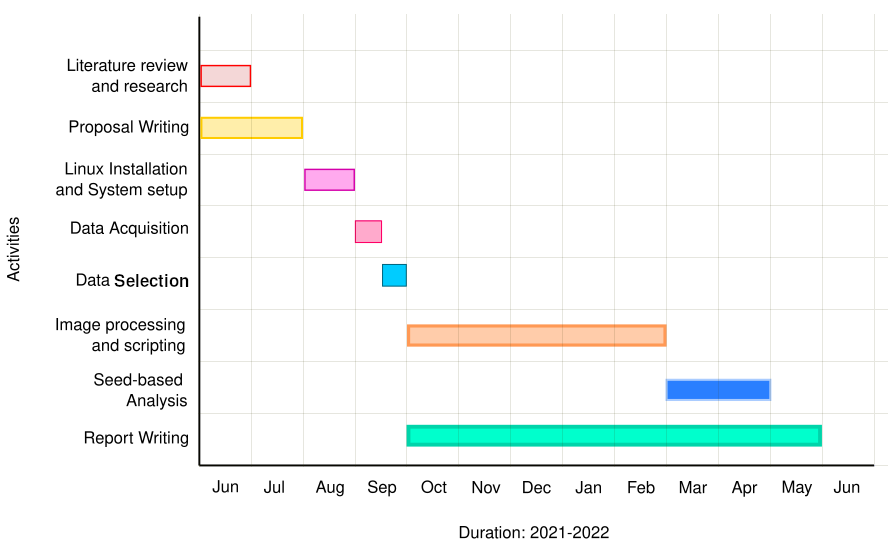
\includegraphics[width=\textwidth]{./.img/proposed-workflow.png}
  \caption{Proposed Workflow (Unchanged)}%
  \label{fig:}
\end{figure}


\end{document}
